\documentclass{report}
\usepackage[final]{pdfpages} %For using cover page pdf in the latex file
\usepackage[utf8]{inputenc}
\usepackage{geometry}
\usepackage{amsmath}
\usepackage{amsthm}
\usepackage{amsfonts}
\usepackage{amssymb}
\usepackage{graphicx}
\usepackage{tocloft}

%\usepackage{perpage} %the perpage package
%\MakePerPage{footnote} %the perpage package command

% For adding TOC in pdf bookmarks
\usepackage{hyperref}
\hypersetup{pdftex,colorlinks=true,allcolors=black}
\usepackage{hypcap}
%
\usepackage{float}
\usepackage{xepersian}
\usepackage{bidi}


\settextfont{Yas}
\SepMark{-}

\renewcommand{\cftsecleader}{\cftdotfill{\cftdotsep}}

\theoremstyle{definition}
\newtheorem{definition}{تعریف}

\title{طرح پیشنهادی پروژه کارشناسی}
\author{امیر حقیقتی ملکی}
\date{پاییز ۹۶}
	
\begin{document}
	%%%%%%%%%%%%%%%%%%%%%%%%%%%%%%%
	%%	 TITLE PAGE - BEGIN	     %%
	%%%%%%%%%%%%%%%%%%%%%%%%%%%%%%%
	\newgeometry{margin=1in}
	\pagenumbering{gobble}
	\begin{titlepage}
				\centering
		
\includegraphics[width=0.25\textwidth]{Resources/logo.png}\par\vspace{1cm}
		{\scshape\LARGE دانشگاه صنعتی امیرکبیر \par}
		{\scshape\LARGE دانشکده مهندسی کامپیوتر و فناوری اطلاعات \par}
		\vspace{1cm}
		{\scshape\Large
			بررسی طرح کلی پروژه کارشناسی
			\par}
		\vspace{1.5cm}
		{\huge\bfseries 
			پیاده‌سازی سامانه‌ای مبتنی بر وب برای سنجش کارایی رابط کاربری وب‌اپلیکیشن‌ها به روش جمع‌سپاری
			\par}
		\vspace{2cm}
		نگارنده:\par
		{\Large امیر حقیقتی ملکی\par}
		\href{mailto:amirh@aut.ac.ir}{amirh@aut.ac.ir}
		\vfill
		استاد راهنما:\par
		{\Large استاد احمد عبداله‌زاده بارفروش\par}
		\href{mailto:ahmad@ce.aut.ac.ir}{ahmad@ce.aut.ac.ir}
		\vfill
		
		% Bottom of the page
		{\large \rl{
				تابستان ۹۷
			}\par}
		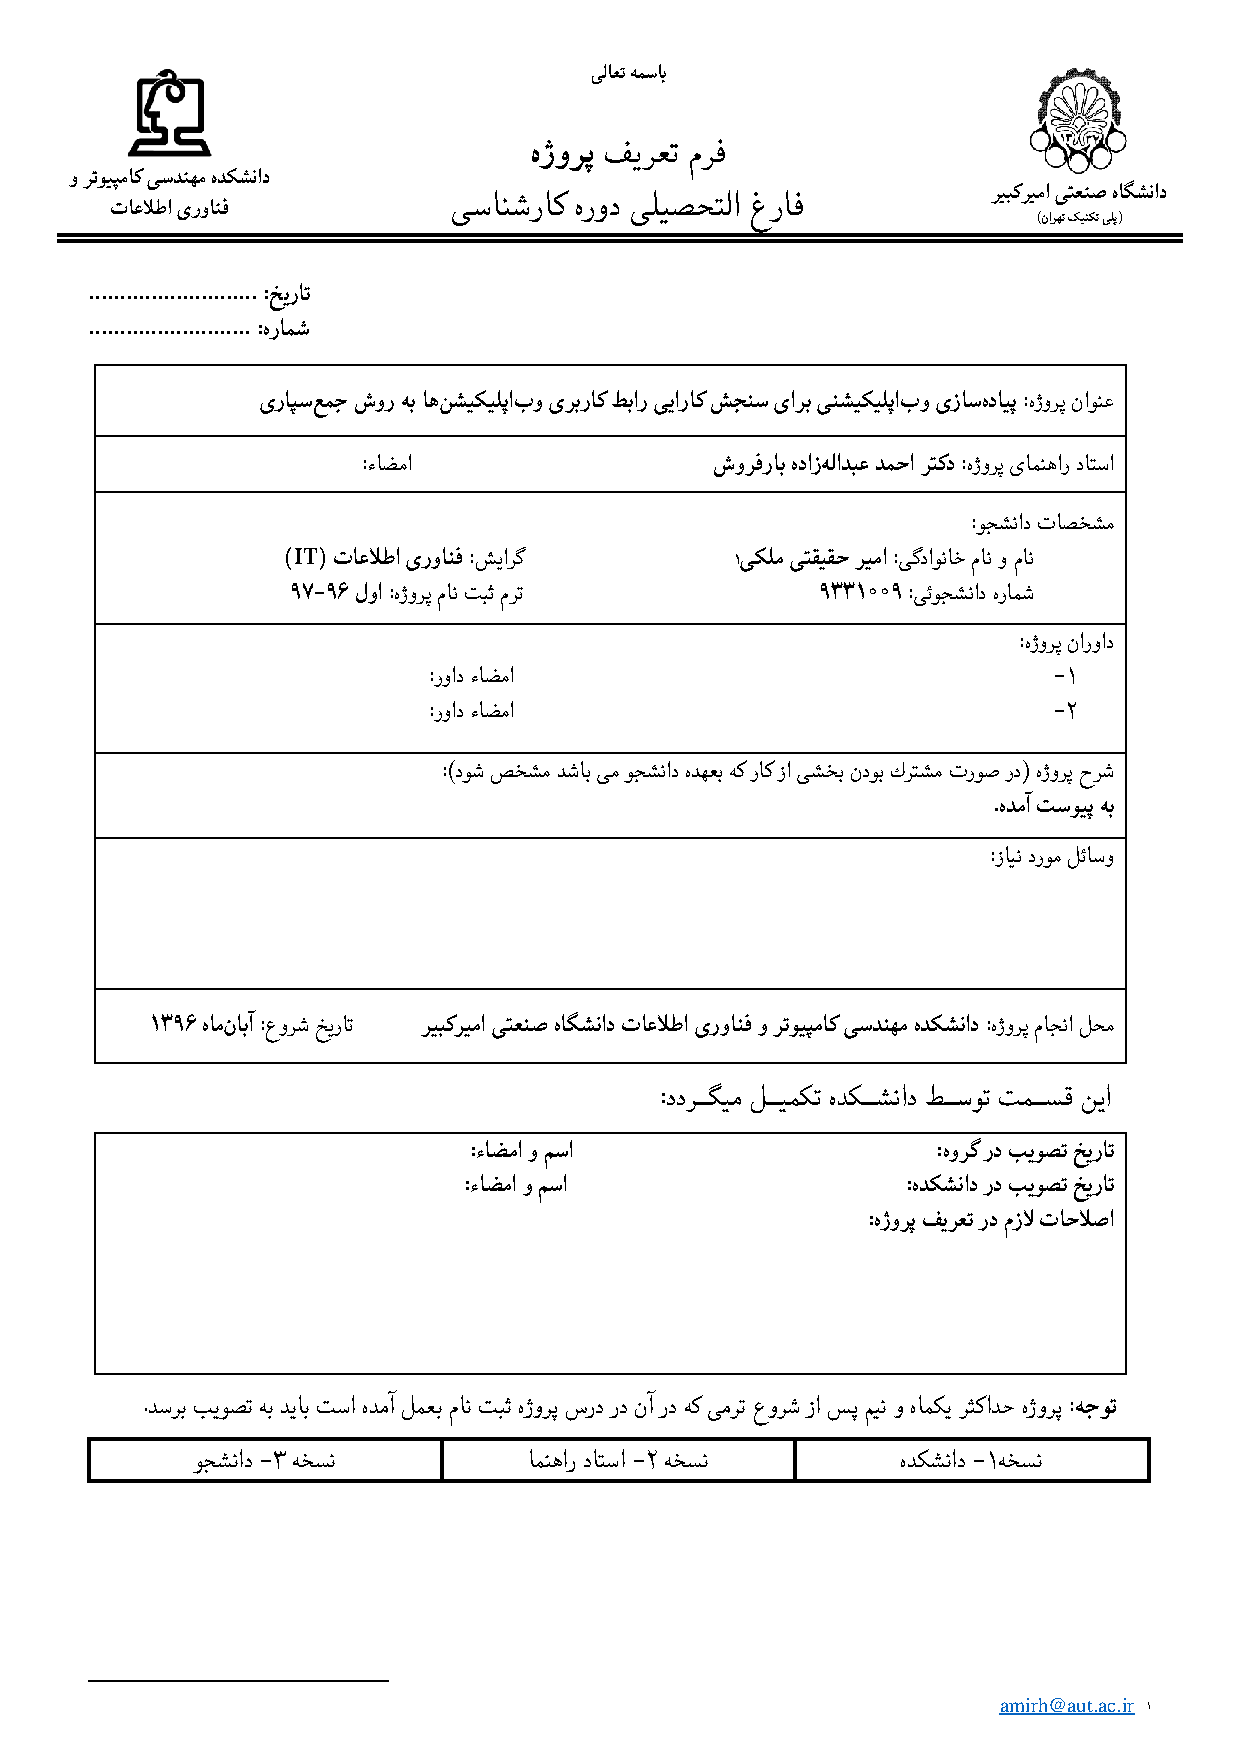
\includepdf[pages=-]{Project_Definition_Page.pdf}
	\end{titlepage}
	\newpage
	\pagenumbering{Alph}
	\begin{abstract}
		\thispagestyle{plain}
		لورم ایپسوم متن ساختگی با تولید سادگی نامفهوم از صنعت چاپ و با استفاده از طراحان گرافیک است. چاپگرها و متون بلکه روزنامه و مجله در ستون و سطرآنچنان که لازم است و برای شرایط فعلی تکنولوژی مورد نیاز و کاربردهای متنوع با هدف بهبود ابزارهای کاربردی می باشد. کتابهای زیادی در شصت و سه درصد گذشته، حال و آینده شناخت فراوان جامعه و متخصصان را می طلبد تا با نرم افزارها شناخت بیشتری را برای طراحان رایانه ای علی الخصوص طراحان خلاقی و فرهنگ پیشرو در زبان فارسی ایجاد کرد. در این صورت می توان امید داشت که تمام و دشواری موجود در ارائه راهکارها و شرایط سخت تایپ به پایان رسد وزمان مورد نیاز شامل حروفچینی دستاوردهای اصلی و جوابگوی سوالات پیوسته اهل دنیای موجود طراحی اساسا مورد استفاده قرار گیرد.
	\end{abstract}
	\newpage
	\pagenumbering{gobble}
	\tableofcontents
	\newpage
	\pagenumbering{arabic}
	\chapter{مقدمه}
	فرایند تولید وب‌اپلیکیشن‌ها به سبب زیبایی فرایند بیسار هزینه‌بری بوده و نیازمنده صرف دقت فراوان است. تست و سنجش نرم‌افزار در متدولوژی‌های رایج و متداول مهندسی نرم‌افزار، یک نوع فعالیت چتری\footnote{Umbrella Activity} به حساب می‌آید به طوری که در تمامی مراحل، اجرای تست‌های مختلف و آزمون‌های گوناگون، به منظور تضمین کیفیت لازم در محصول نهایی، می‌بایست انجام شود.
	\section{قسمت اول}
	
\end{document}